% !TeX spellcheck = cs_CZ
\wikitextrule
\begin{example}\label{MAI:exam020} 
  Rovnice $x=\cos t,\ y=\sin t\quad t\in\langle0,\pi\rangle$, definují parametricky funkci 
  \begin{equation}
    f: y= \sqrt{1-x^2}, \quad x\in\langle-1,1\rangle,
  \end{equation}
  jejíž grafem je polokružnice, ležící v horní polorovině $\{(x,y)\in\realset^2, y\geq0\}$.
  
  {\centering
   \captionsetup{type=figure}
%   % !TeX spellcheck = cs_CZ
%Graf funkce \(y=\sqrt{1-x^2}\) je polokružnice

\documentclass[11pt]{standalone}
\usepackage{xltxtra}
\usepackage[usenames,x11names]{xcolor}
\usepackage{tikz}
\usepackage{pgfplots}
  \pgfplotsset{compat=newest}
\usepackage{amsmath}

\begin{document}
  \begin{tikzpicture}[thick,scale=0.7, every node/.style={transform shape}]
    \begin{axis}[
      xmin = -1.2, xmax = 1.2, ymin = 0, ymax = 1.3,  % osy
      domain = -1:1,
      restrict y to domain=0:1,
      unit vector ratio=1 1 1,  % axis equal
      grid = major,   % both
      grid style={line width=.1pt, draw=gray!20},
      major grid style={dashed, line width=.2pt, draw=gray!40},
      minor tick num=5,
      clip = true,
      clip mode=individual,
      axis x line = middle,
      axis y line = middle,
      xlabel={\(x\)}, ylabel={\(y\)},
      enlarge y limits={rel=0.07},
      enlarge x limits={rel=0.07},
    ]
    
      \addplot[color=Gold3, samples=200, smooth, ultra thick, unbounded coords=jump, no markers] 
         gnuplot{sqrt(1-x^2)};  
    \end{axis}
  \end{tikzpicture} 
\end{document}
   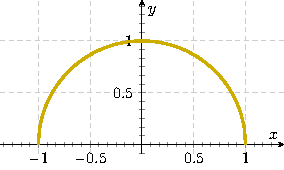
\includegraphics[width=0.5\linewidth]{mai_fig008.pdf}
   \captionof{figure}{Graf funkce \(y=\sqrt{1-x^2}\) je polokružnice}
   \label{mai_fig008}
  \par}
\end{example}